\documentclass[11pt]{article}

\newcommand{\yourname}{}
\newcommand{\yourcollaborators}{}

\def\comments{0}

%format and packages

%\usepackage{algorithm, algorithmic}
\usepackage{algpseudocode}
\usepackage{amsmath, amssymb, amsthm}
\usepackage{enumerate}
\usepackage{enumitem}
\usepackage{framed}
\usepackage{verbatim}
\usepackage[margin=1.0in]{geometry}
\usepackage{microtype}
\usepackage{kpfonts}
\usepackage{graphicx}       % upload image
\usepackage{palatino}
	\DeclareMathAlphabet{\mathtt}{OT1}{cmtt}{m}{n}
	\SetMathAlphabet{\mathtt}{bold}{OT1}{cmtt}{bx}{n}
	\DeclareMathAlphabet{\mathsf}{OT1}{cmss}{m}{n}
	\SetMathAlphabet{\mathsf}{bold}{OT1}{cmss}{bx}{n}
	\renewcommand*\ttdefault{cmtt}
	\renewcommand*\sfdefault{cmss}
	\renewcommand{\baselinestretch}{1.06}
\usepackage[usenames,dvipsnames]{xcolor}
\definecolor{DarkGreen}{rgb}{0.15,0.5,0.15}
\definecolor{DarkRed}{rgb}{0.6,0.2,0.2}
\definecolor{DarkBlue}{rgb}{0.2,0.2,0.6}
\definecolor{DarkPurple}{rgb}{0.4,0.2,0.4}
\usepackage[pdftex]{hyperref}
\hypersetup{
	linktocpage=true,
	colorlinks=true,				% false: boxed links; true: colored links
	linkcolor=DarkBlue,		% color of internal links
	citecolor=DarkBlue,	% color of links to bibliography
	urlcolor=DarkBlue,		% color of external links
}

\usepackage[boxruled,vlined,nofillcomment]{algorithm2e}
	\SetKwProg{Fn}{Function}{\string:}{}
	\SetKwFor{While}{While}{}{}
	\SetKwFor{For}{For}{}{}
	\SetKwIF{If}{ElseIf}{Else}{If}{:}{ElseIf}{Else}{:}
	\SetKw{Return}{Return}
	
\usepackage{pdfpages}
%enclosure macros
\newcommand{\paren}[1]{\ensuremath{\left( {#1} \right)}}
\newcommand{\bracket}[1]{\ensuremath{\left\{ {#1} \right\}}}
\renewcommand{\sb}[1]{\ensuremath{\left[ {#1} \right\]}}
\newcommand{\ab}[1]{\ensuremath{\left\langle {#1} \right\rangle}}

%probability macros
\newcommand{\ex}[2]{{\ifx&#1& \mathbb{E} \else \underset{#1}{\mathbb{E}} \fi \left[#2\right]}}
\newcommand{\pr}[2]{{\ifx&#1& \mathbb{P} \else \underset{#1}{\mathbb{P}} \fi \left[#2\right]}}
\newcommand{\var}[2]{{\ifx&#1& \mathrm{Var} \else \underset{#1}{\mathrm{Var}} \fi \left[#2\right]}}

%useful CS macros
\newcommand{\poly}{\mathrm{poly}}
\newcommand{\polylog}{\mathrm{polylog}}
\newcommand{\zo}{\{0,1\}}
\newcommand{\pmo}{\{\pm1\}}
\newcommand{\getsr}{\gets_{\mbox{\tiny R}}}
\newcommand{\card}[1]{\left| #1 \right|}
\newcommand{\set}[1]{\left\{#1\right\}}
\newcommand{\negl}{\mathrm{negl}}
\newcommand{\eps}{\varepsilon}
\DeclareMathOperator*{\argmin}{arg\,min}
\DeclareMathOperator*{\argmax}{arg\,max}
\newcommand{\eqand}{\qquad \textrm{and} \qquad}
\newcommand{\ind}[1]{\mathbb{I}\{#1\}}
\newcommand{\sslash}{\ensuremath{\mathbin{/\mkern-3mu/}}}

%mathbb
\newcommand{\N}{\mathbb{N}}
\newcommand{\R}{\mathbb{R}}
\newcommand{\Z}{\mathbb{Z}}
%mathcal
\newcommand{\cA}{\mathcal{A}}
\newcommand{\cB}{\mathcal{B}}
\newcommand{\cC}{\mathcal{C}}
\newcommand{\cD}{\mathcal{D}}
\newcommand{\cE}{\mathcal{E}}
\newcommand{\cF}{\mathcal{F}}
\newcommand{\cL}{\mathcal{L}}
\newcommand{\cM}{\mathcal{M}}
\newcommand{\cO}{\mathcal{O}}
\newcommand{\cP}{\mathcal{P}}
\newcommand{\cQ}{\mathcal{Q}}
\newcommand{\cR}{\mathcal{R}}
\newcommand{\cS}{\mathcal{S}}
\newcommand{\cU}{\mathcal{U}}
\newcommand{\cV}{\mathcal{V}}
\newcommand{\cW}{\mathcal{W}}
\newcommand{\cX}{\mathcal{X}}
\newcommand{\cY}{\mathcal{Y}}
\newcommand{\cZ}{\mathcal{Z}}

%theorem macros
\newtheorem{thm}{Theorem}
\newtheorem{lem}[thm]{Lemma}
\newtheorem{fact}[thm]{Fact}
\newtheorem{clm}[thm]{Claim}
\newtheorem{rem}[thm]{Remark}
\newtheorem{coro}[thm]{Corollary}
\newtheorem{prop}[thm]{Proposition}
\newtheorem{conj}[thm]{Conjecture}

\theoremstyle{definition}
\newtheorem{defn}[thm]{Definition}


\newcommand{\instructor}{Virgil Pavlu}
\newcommand{\hwnum}{12}
\newcommand{\hwdue}{Wednesday, May 20 at 11:59pm via \href{https://gradescope.com/courses/229309}{Gradescope}}

\theoremstyle{theorem}
\newtheorem{prob}{}
\newtheorem{sol}{Solution}

\definecolor{cit}{rgb}{0.05,0.2,0.45} 
\newcommand{\solution}{\medskip\noindent{\color{DarkBlue}\textbf{Solution:}}}

\begin{document}
{\Large 
\begin{center}{CS5800: Algorithms} --- Spring '21 --- \instructor \end{center}}
{\large
\vspace{10pt}
\noindent Homework~\hwnum \vspace{2pt}\\
Submit via \href{https://www.gradescope.com/courses/232127}{Gradescope}}

\bigskip
{\large \noindent Name: Xuran Feng }

{\large \noindent Collaborators: \yourcollaborators}

\vspace{15pt}

{\large \noindent Instructions:}

\begin{itemize}

\item Make sure to put your name on the first page.  If you are using the \LaTeX~template we provided, then you can make sure it appears by filling in the \texttt{yourname} command.

\item Please review the grading policy outlined in the course information page.

\item You must also write down with whom you worked on the assignment.  If this changes from problem to problem, then you should write down this information separately with each problem.

\item Problem numbers (like Exercise 3.1-1) are corresponding to CLRS $3^{rd}$ edition.  While the  $2^{nd}$ edition  has  similar  problems  with  similar  numbers,  the  actual  exercises  and their solutions are different, so make sure you are using the $3^{rd}$ edition.

\end{itemize}

\newpage

\begin{prob} \textbf{(20 points)} Exercise 26.1-3.
\end{prob}
\solution
If there is no path $s\sim u\sim t$, there are three cases that there is no path $s\sim u$ or there is no path $u\sim t$. If there is no path $s\sim u$, then there should be no flow coming into u for all vertices v because all vertices connected to u should also have no path with s else there would be a path $s\sim u$, there is also no water coming out of u since vertex doesn't store water. Similarly, if it is the second case where the path $u\sim t$ doesn't exist, although u may have access to source and have a positive flow coming into itself, since vertex doesn't store water, u must send water out to other vertices, but other vertices cannot have a path with t else it would violate the assumption that there is no path $u\sim t$, so there must be no water coming out of vertex u because the water has no place to be stored, accordingly there is also no water coming into vertex u. In both cases, the maximum flow will never choose u as an intermediate and for all vertices v f(u,v)==f(v,u)=0 must be valid.
\begin{prob} \textbf{(20 points)} Exercise 26.1-4.
\end{prob}
\solution
According to the textbook, a flow in G that satisfies two properties: capacity constraint, $0\leq f(u, v)\leq c(u, v)$; flow conservation, $\sum f(v,u)=\sum f(u,v)$. We need to show that $\alpha f_1+(1-\alpha)f_2$ also satisfies these two properties. Because $0\leq f_1\leq c$ and $0\leq f_2\leq c$, so $\alpha f_1+(1-\alpha)f_2\geq \alpha \cdot 0+(1-\alpha)\cdot 0 \geq 0$, $\alpha f_1+(1-\alpha)f_2\leq \alpha \cdot c+(1-\alpha)\cdot c \leq c$, thus the first property is satisfied. For the second property, $\sum f_1(v,u)=\sum f_1(u,v)$ and $\sum f_2(v,u)=\sum f_2(u,v)$ are satisfied, $\sum(\alpha f_1(v,u)+(1-\alpha)f_2(v,u))$=$\alpha\cdot\sum f_1(v,u)+(1-\alpha)\cdot\sum f_2(v,u)$=$\alpha\cdot\sum f_1(u,v)+(1-\alpha)\cdot\sum f_2(u,v)$=$\sum(\alpha f_1(u,v)+(1-\alpha)f_2(u,v))$, thus the second property is also satisfied, so $\alpha f_1+(1-\alpha)f_2$ is also a flow of G.
\begin{prob} \textbf{(20 points)} Exercise 26.2-2.
\end{prob}
\solution
The flow across the cut is f(s,$v_1$)+f($v_2$,$v_1$)+f($v_4$,$v_3$)+f($v_4$,t)-f($v_3$,$v_2$)=11+1+7+4-4=19, the capacity of this cut is  c(s,$v_1$)+c($v_2$,$v_1$)+c($v_4$,$v_3$)+c($v_4$,t)=16+4+7+4=31.
\begin{prob} \textbf{(Extra Credit)} Exercise 26.2-10.
\end{prob}
\solution

\begin{prob} \textbf{(30 points)} Implement Push-Relabel for finding maximum flow.

Extra Credit: use relabel-to-front idea from Chapter 26.5 with the Discharge procedure.
\end{prob}
\solution
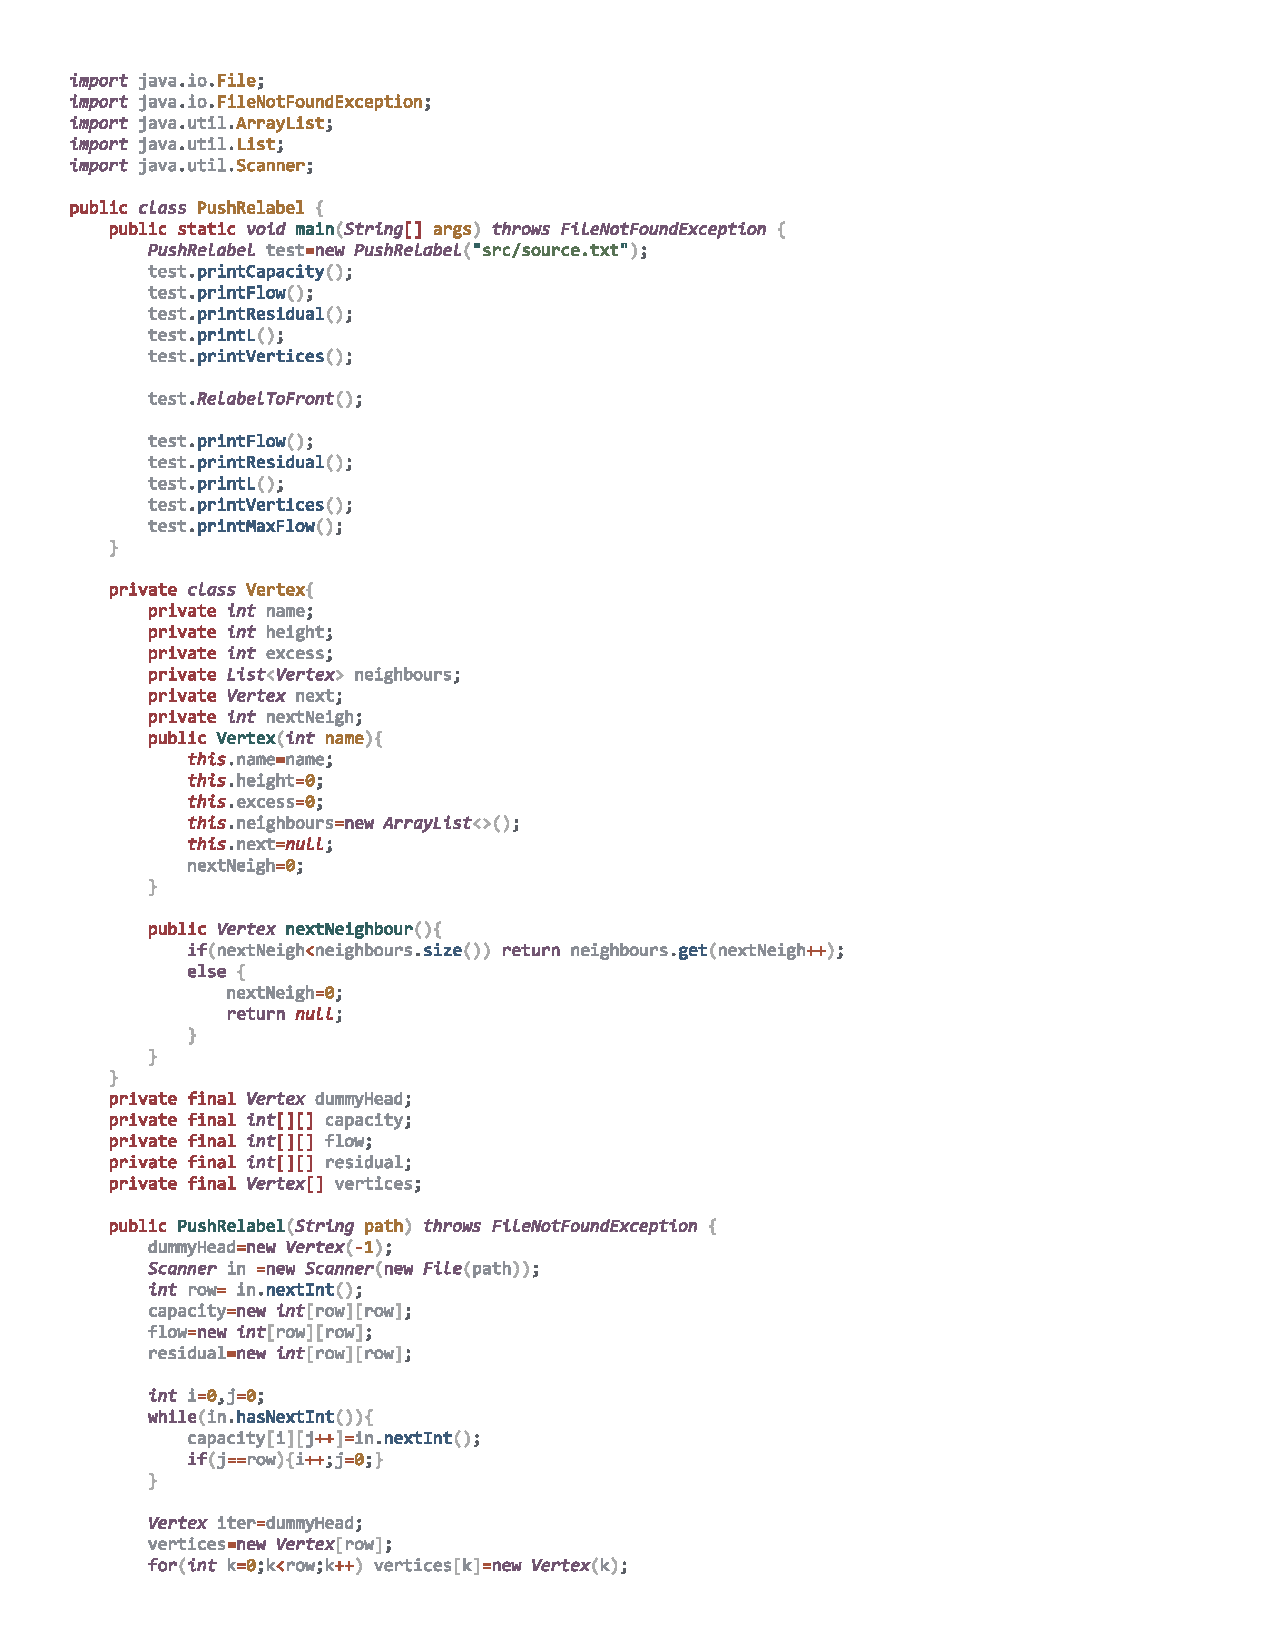
\includepdf[pages=-,pagecommand={},width=\textwidth]{Code.pdf}
\begin{prob} \textbf{(15 points)} Explain in a brief paragraph the following sentence from textbook page 737: “To make the preflow a legal flow, the algorithm then sends the excess collected in the reservoirs of overflowing vertices back to the source by continuing to relabel vertices to above the fixed height $|V|$ of the source”.
\end{prob}
\solution
The source vertex is assigned a fixed height $|V|$ to make sure flowing back to source vertex is the last choice when flowing into sink is not possible but there is still water stored in the intermediate vertices. When intermediate vertices find no way to flow into the sink and the water simply cycle between intermediate vertices, to end the loop we need to find somewhere to clear reservoirs, and one choice is to flow back to source; to flow back to source, we need to relabel vertices above source's height which is $|V|$, since the intermedaite vertices' heights are above $|V|$, the extra flow stored in intermediate vertices can flow back into source, the flow matrix will become a valid one else the flow conservation will be violated at the end.
\begin{prob} \textbf{(Extra Credit)} Exercise 26.4.4.
\end{prob}
\solution

\end{document}